\documentclass[11pt]{article}
\usepackage{amsmath}
\usepackage{amssymb}
\usepackage{graphicx}
\usepackage{tabularx}
\usepackage{fancyhdr}
\usepackage{lastpage}

% Page layout
\usepackage[top=1in, bottom=1in, left=1in, right=1in]{geometry}

% Header and footer
\pagestyle{fancy}
\fancyhf{}
\rfoot{Page \thepage}
\renewcommand{\headrulewidth}{0pt}

% Modified Question command with left-aligned number
\newcommand{\questiona}[2]{
    \noindent\textbf{Q#2.} #1 \hfill \textbf{[1 Mark]}
}

\newcommand{\questionb}[2]{
    \noindent\textbf{Q#2.} #1 \hfill \textbf{[2 Marks]}
}

\begin{document}

% Title section with horizontal line
\begin{center}
    \Large\textbf{GATE 2017 - Electrical Engineering (EE)} \\
    \large\textbf{General Aptitude and Technical Questions} \\
    \rule{\textwidth}{0.5pt} % Horizontal line below heading
\end{center}

\vspace{0.5cm}

\section*{General Aptitude}

\questiona{After Rajendra Chola returned from his voyage to Indonesia, he \_\_\_\_\_ to visit the temple in Thanjavur.}{1}
\begin{enumerate}
    \item[(A)] was wishing  
    \item[(B)] is wishing  
    \item[(C)] wished  
    \item[(D)] had wished  
\end{enumerate}
\vspace{0.5cm}

\questiona{Research in the workplace reveals that people work for many reasons \_\_\_\_\_.}{2}
\begin{enumerate}
    \item[(A)] money beside  
    \item[(B)] beside money  
    \item[(C)] money besides  
    \item[(D)] besides money  
\end{enumerate}
\vspace{0.5cm}

\questiona{Rahul, Murali, Srinivas and Arul are seated around a square table. Rahul is sitting to the left of Murali. Srinivas is sitting to the right of Arul. Which of the following pairs are seated opposite each other?}{3}
\begin{enumerate}
    \item[(A)] Rahul and Murali  
    \item[(B)] Srinivas and Arul  
    \item[(C)] Srinivas and Murali  
    \item[(D)] Srinivas and Rahul  
\end{enumerate}
\vspace{0.5cm}

\questiona{Find the smallest number \( y \) such that \( y \times 162 \) is a perfect cube.}{4}
\begin{enumerate}
    \item[(A)] 24  
    \item[(B)] 27  
    \item[(C)] 32  
    \item[(D)] 36  
\end{enumerate}
\vspace{0.5cm}

\questiona{The probability that a 3-digit number does NOT contain the digits 0, 5, or 9 is}{5}
\begin{enumerate}
    \item[(A)] 0.3\%  
    \item[(B)] 0.6\%  
    \item[(C)] 0.7\%  
    \item[(D)] 0.9\%  
\end{enumerate}
\vspace{0.5cm}

\questionb{“The hold of the nationalist imagination on our colonial past is such that anything inadequately or improperly nationalist is just not history.”\\
Which of the following statements best reflects the author’s opinion?}{6}
\begin{enumerate}
    \item[(A)] Nationalists are highly imaginative.  
    \item[(B)] History is viewed through the filter of nationalism.  
    \item[(C)] Our colonial past never happened.  
    \item[(D)] Nationalism has to be both adequately and properly imagined.  
\end{enumerate}
\vspace{0.5cm}

\questionb{Six people are seated around a circular table. There are at least two men and two women. There are at least three right-handed persons. Every woman has a left-handed person to her immediate right. None of the women are right-handed. The number of women at the table is}{7}
\begin{enumerate}
    \item[(A)] 2  
    \item[(B)] 3  
    \item[(C)] 4  
    \item[(D)] Cannot be determined  
\end{enumerate}
\vspace{0.5cm}

\questionb{The expression \( g(x, y) = |x - y| + |x + y| \) is equal to}{8}
\begin{enumerate}
    \item[(A)] the maximum of \( x \) and \( y \)  
    \item[(B)] the minimum of \( x \) and \( y \)  
    \item[(C)] \( 2 \max(x, y) \)  
    \item[(D)] none of the above  
\end{enumerate}
\vspace{0.5cm}

\questionb{Arun, Gulab, Neel and Shweta must choose one shirt each from a pile of four shirts coloured red, pink, blue and white respectively. Arun dislikes the colour red and Shweta dislikes the colour white. Gulab and Neel like all the colours. In how many different ways can they choose the shirts so that no one has a shirt with a colour he or she dislikes?}{9}
\begin{enumerate}
    \item[(A)] 21  
    \item[(B)] 18  
    \item[(C)] 16  
    \item[(D)] 14  
\end{enumerate}
\vspace{0.5cm}

\questionb{A contour line joins locations having the same height above the mean sea level. The following is a contour plot of a geographical region. Contour lines are shown at 25 m intervals in this plot. If in a flood, the water level rises to 525 m, which of the villages P, Q, R, S, T get submerged?}{10}
\begin{center}
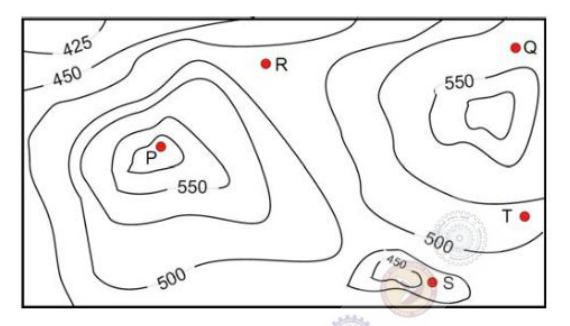
\includegraphics[width=0.5\textwidth]{figures/10.png}
\end{center}
\begin{enumerate}
    \item[(A)] P, Q  
    \item[(B)] P, Q, T  
    \item[(C)] R, S, T  
    \item[(D)] Q, R, S  
\end{enumerate}
\vspace{0.5cm}

\section*{Technical Section}

\questiona{The matrix \( A = \begin{bmatrix} 0 & -1 & 0 \\ 10 & 3 & 1 \\ 2 & 0 & 2 \end{bmatrix} \) has three distinct eigenvalues and one of its eigenvectors is \( \begin{bmatrix} 0 \\ 1 \\ -1 \end{bmatrix} \). Which one of the following can be another eigenvector of \( A \)?}{1}
\begin{enumerate}
    \item[(A)] \( \begin{bmatrix} 0 \\ -1 \\ 1 \end{bmatrix} \)  
    \item[(B)] \( \begin{bmatrix} 0 \\ 0 \\ 1 \end{bmatrix} \)  
    \item[(C)] \( \begin{bmatrix} -1 \\ 0 \\ -1 \end{bmatrix} \)  
    \item[(D)] \( \begin{bmatrix} 1 \\ 1 \\ 1 \end{bmatrix} \)  
\end{enumerate}
\vspace{0.5cm}

\questiona{For a complex number \( z \), \begin{center}
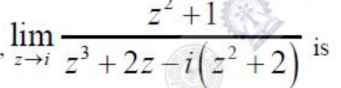
\includegraphics[width=0.2\textwidth]{figures/2.png}
\end{center}}{2}
\begin{enumerate}
    \item[(A)] \(-2i\)  
    \item[(B)] \(-i\)  
    \item[(C)] \(i\)  
    \item[(D)] \(2i\)  
\end{enumerate}
\vspace{0.5cm}

\questiona{Let \( z(t) = x(t) * y(t) \), where “\(*\)” denotes convolution. Let \( c \) be a positive real-valued constant. Choose the correct expression for \( z(ct) \).}{3}
\begin{enumerate}
    \item[(A)] \( c \cdot x(ct) * y(ct) \)  
    \item[(B)] \( x(ct) * y(ct) \)  
    \item[(C)] \( c \cdot x(t) * y(ct) \)  
    \item[(D)] \( c \cdot x(ct) * y(t) \)  
\end{enumerate}
\vspace{0.5cm}

\questiona{A solid iron cylinder is placed in a region containing a uniform magnetic field such that the cylinder axis is parallel to the magnetic field direction. The magnetic field lines inside the cylinder will}{4}
\begin{enumerate}
    \item[(A)] bend closer to the cylinder axis  
    \item[(B)] bend farther away from the axis  
    \item[(C)] remain uniform as before  
    \item[(D)] cease to exist inside the cylinder  
\end{enumerate}
\vspace{0.5cm}

\questiona{Consider an electron, a neutron and a proton initially at rest and placed along a straight line such that the neutron is exactly at the center of the line joining the electron and proton. At \( t = 0 \), the particles are released but are constrained to move along the same straight line. Which of these will collide first?}{5}
\begin{enumerate}
    \item[(A)] The particles will never collide  
    \item[(B)] All will collide together  
    \item[(C)] Proton and neutron  
    \item[(D)] Electron and neutron  
\end{enumerate}
\vspace{0.5cm}

\questiona{The transfer function of a system is given by,\\
\[
\frac{V_o(s)}{V_i(s)} = \frac{1 - s}{1 + s}
\] 
Let the output of the system be \( v_o(t) = V_o \sin(\omega t + \phi) \) for the input, \( v_i(t) = V_i \sin(\omega t) \). Then the minimum and maximum values of \( \phi \) (in radians) are respectively}{6}
\begin{enumerate}
    \item[(A)] \( \frac{\pi}{2} \) and \( \frac{\pi}{2} \)  
    \item[(B)] \( \frac{\pi}{2} \) and 0  
    \item[(C)] 0 and \( \frac{\pi}{2} \)  
    \item[(D)] \(-\pi \) and 0  
\end{enumerate}
\vspace{0.5cm}

\questiona{Consider the system with following input-output relation \\
\( y[n] = x[n] + x[n - 1] \) \\
where, \( x[n] \) is the input and \( y[n] \) is the output. The system is}{7}
\begin{enumerate}
    \item[(A)] invertible and time invariant  
    \item[(B)] invertible and time varying  
    \item[(C)] non-invertible and time invariant  
    \item[(D)] non-invertible and time varying  
\end{enumerate}
\vspace{0.5cm}

\questiona{A 4 pole induction machine is working as an induction generator. The generator supply frequency is 60 Hz. The rotor current frequency is 5 Hz. The mechanical speed of the rotor in RPM is}{8}
\begin{enumerate}
    \item[(A)] 1350  
    \item[(B)] 1650  
    \item[(C)] 1950  
    \item[(D)] 2250  
\end{enumerate}
\vspace{0.5cm}

\questiona{A source is supplying a load through a 2-phase, 3-wire transmission system as shown in figure below. The instantaneous voltage and current in phase-a are \( v_a = 220\sin(100\pi t) \) V and \( i_a = 10\sin(100\pi t) \) A respectively. Similarly for phase-b, the instantaneous voltage and current are \( v_b = 220\cos(100\pi t) \) V and \( i_b = 10\cos(100\pi t) \) A, respectively. The total instantaneous power flowing from the source to the load is}{9}
\begin{center}
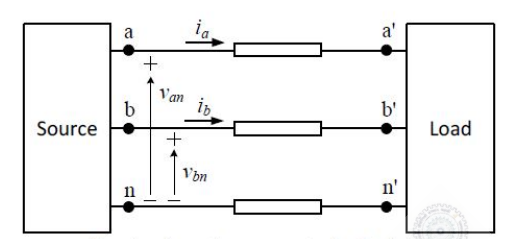
\includegraphics[width=0.5\textwidth]{figures/9.png}
\end{center}
\begin{enumerate}
    \item[(A)] 2200 W  
    \item[(B)] \( 2200\sin^2(100\pi t) \) W  
    \item[(C)] 4400 W  
    \item[(D)] \( 2200\sin(100\pi t)\cos(100\pi t) \) W  
\end{enumerate}
\vspace{0.5cm}

\questiona{A 3-bus power system is shown in the figure below, where the diagonal elements of Y-bus matrix are: \( Y_{11} = -j12 \) pu, \( Y_{22} = -j15 \) pu and \( Y_{33} = -j7 \) pu. The per unit values of the line reactances \( p, q \) and \( r \) shown in the figure are}{10}
\begin{center}
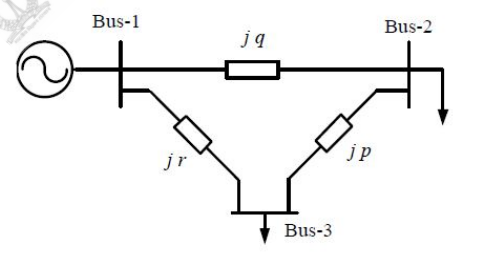
\includegraphics[width=0.5\textwidth]{figures/10a.png}
\end{center}
\begin{enumerate}
    \item[(A)] \( p = -0.2, q = -0.1, r = -0.5 \)  
    \item[(B)] \( p = 0.2, q = 0.1, r = 0.5 \)  
    \item[(C)] \( p = -5, q = -10, r = -2 \)  
    \item[(D)] \( p = 5, q = 10, r = 2 \)  
\end{enumerate}
\vspace{0.5cm}

\questiona{A closed loop system has the characteristic equation given by \( s^3 + Ks^2 + (K + 2)s + 3 = 0 \). For this system to be stable, which one of the following conditions should be satisfied?}{11}
\begin{enumerate}
    \item[(A)] \( K < 0.5 \)  
    \item[(B)] \( 0.5 < K < 1 \)  
    \item[(C)] \( 0 < K < 1 \)  
    \item[(D)] \( K > 1 \)  
\end{enumerate}
\vspace{0.5cm}

\questiona{The slope and level detector circuit in a CRO has a delay of 100 ns. The start-stop sweep generator has a response time of 50 ns. In order to display correctly, a delay line of \_\_\_\_\_\_ has to be inserted into the y-channel.}{12}\\
(A) 150 ns has to be inserted into the y-channel\\
(B) 150 ns has to be inserted into the x-channel\\
(C) 150 ns has to be inserted into both x and y channels\\
(D) 100 ns has to be inserted into both x and y channels\\
\vspace{0.5cm}

\questiona{The Boolean expression \( AB + AC + BC \) simplifies to}{13}
\begin{enumerate}
    \item[(A)] \( BC + AC \)  
    \item[(B)] \( AB + AC + B \)  
    \item[(C)] \( AB + AC \)  
    \item[(D)] \( AB + BC \)  
\end{enumerate}
\vspace{0.5cm}

\questiona{For the circuit shown in the figure below, assume that diodes \( D_1, D_2 \) and \( D_3 \) are ideal. The DC components of voltages \( v_1 \) and \( v_2 \), respectively are}{14}
\begin{center}
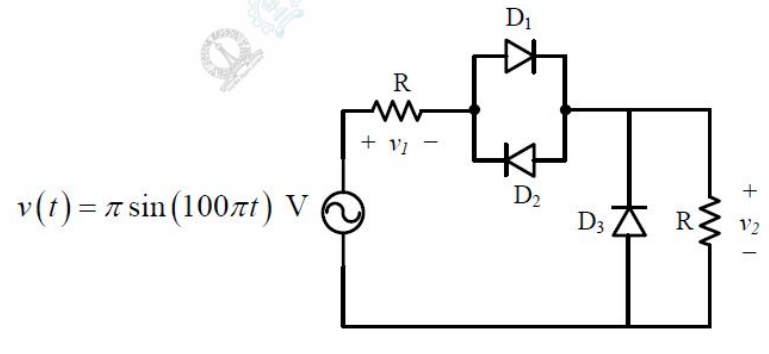
\includegraphics[width=0.5\textwidth]{figures/14.png}
\end{center}
\begin{enumerate}
    \item[(A)] 0 V and 1 V  
    \item[(B)] \(-0.5\) V and 0.5 V  
    \item[(C)] 1 V and 0.5 V  
    \item[(D)] 1 V and 1 V  
\end{enumerate}
\vspace{0.5cm}

\questiona{For the power semiconductor devices IGBT, MOSFET, Diode and Thyristor, which one of the following statements is TRUE?}{15}
\begin{enumerate}
    \item[(A)] All the four are majority carrier devices.  
    \item[(B)] All the four are minority carrier devices.  
    \item[(C)] IGBT and MOSFET are majority carrier devices, whereas Diode and Thyristor are minority carrier devices.  
    \item[(D)] MOSFET is majority carrier device, whereas IGBT, Diode, Thyristor are minority carrier devices.  
\end{enumerate}
\vspace{0.5cm}

\questiona{Consider \( g(t) = 
\begin{cases}
|t|, & t < 0 \\
[t], & t = 0 \\
\lceil t \rceil, & t > 0
\end{cases} \)\\
where \( \lfloor \cdot \rfloor \) represents the largest integer less than or equal to the argument, and \( \lceil \cdot \rceil \) denotes the smallest integer greater than or equal to the argument. The coefficient of the second harmonic component of the Fourier series representing \( g(t) \) is \_\_\_\_\_\_}{16}
\vspace{0.5cm}

\questiona{Let \( I = c \iint_R xy^2 \, dx\,dy \), where \( R \) is the region shown in the figure and \( c = 6 \times 10^5 \). The value of \( I \) equals \_\_\_\_\_\_ (Give the answer up to two decimal places.)}{17}
\begin{center}
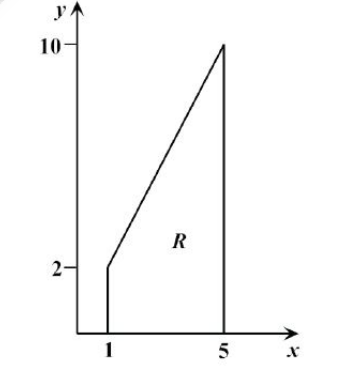
\includegraphics[width=0.5\textwidth]{figures/17.png}
\end{center}
\vspace{0.5cm}

\questiona{The power supplied by the 25 V source in the figure shown below is \_\_\_\_\_\_ W.}{18}
\begin{center}
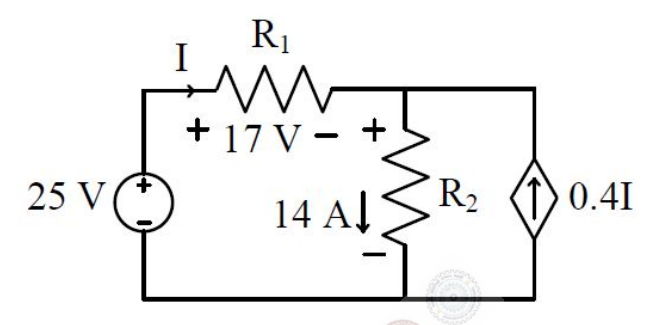
\includegraphics[width=0.5\textwidth]{figures/18.png}
\end{center}
\vspace{0.5cm}

\questiona{The equivalent resistance between the terminals A and B is \_\_\_\_\_\_ \( \Omega \).}{19}
\begin{center}
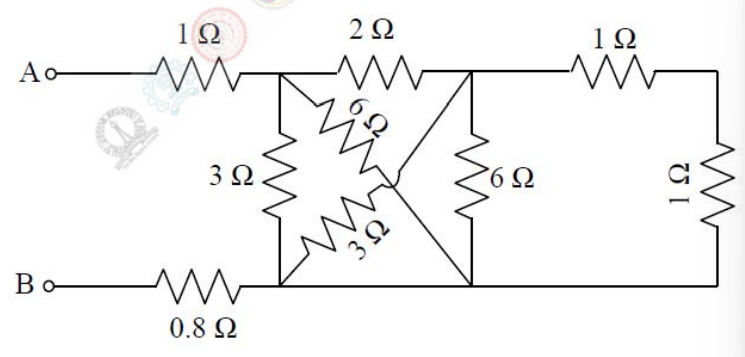
\includegraphics[width=0.5\textwidth]{figures/19.png}
\end{center}
\vspace{0.5cm}

\questiona{A three-phase, 50 Hz, star-connected cylindrical-rotor synchronous machine is running as a motor. The machine is operated from a 6.6 kV grid and draws current at unity power factor (UPF). The synchronous reactance of the motor is 30 \( \Omega \) per phase. The load angle is \( 30^\circ \). The power delivered to the motor in kW is \_\_\_\_\_\_ (Give the answer up to one decimal place).}{20}
\vspace{0.5cm}

\questiona{A 10-bus power system consists of four generator buses indexed as G1, G2, G3, G4 and six load buses indexed as L1, L2, L3, L4, L5, L6. The generator-bus G1 is considered as slack bus, and the load buses L3 and L4 are voltage controlled buses. The generator at bus G2 cannot supply the required reactive power demand, and hence it is operating at its maximum reactive power limit. The number of non-linear equations required for solving the load flow problem using Newton-Raphson method in polar form is \_\_\_\_\_\_}{21}
\vspace{0.5cm}

\questiona{Consider the unity feedback control system shown. The value of \( K \) that results in a phase margin of the system to be \( 30^\circ \) is \_\_\_\_\_\_ (Give the answer up to two decimal places.)}{22}
\begin{center}
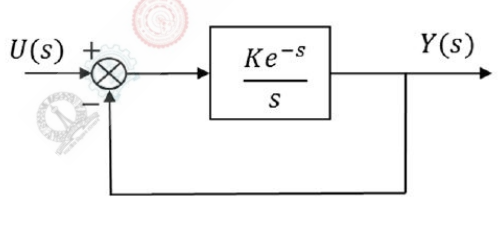
\includegraphics[width=0.5\textwidth]{figures/22.png}
\end{center}
\vspace{0.5cm}

\questiona{The following measurements are obtained on a single phase load: \( V = 220 \) V \( \pm 1\% \), \( I = 5.0 \) A \( \pm 1\% \) and \( W = 555 \) W \( \pm 2\% \). If the power factor is calculated using these measurements, the worst case error in the calculated power factor in percent is \_\_\_\_\_\_ (Give answer up to one decimal place.)}{23}
\vspace{0.5cm}

\questiona{In the converter circuit shown below, the switches are controlled such that the load voltage \( v_o(t) \) is a 400 Hz square wave. The RMS value of the fundamental component of \( v_o(t) \) in volts is \_\_\_\_\_\_}{24}
\begin{center}
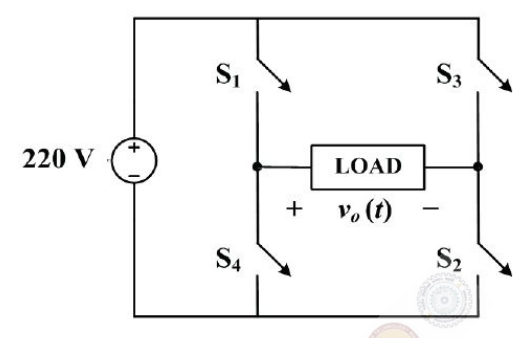
\includegraphics[width=0.5\textwidth]{figures/24.png}
\end{center}
\vspace{0.5cm}

\questiona{A 3-phase voltage source inverter is supplied from a 600 V DC source as shown in the figure below. For a star connected resistive load of 20 \( \Omega \) per phase, the load power for 120° device conduction, in kW, is \_\_\_\_\_\_}{25}
\begin{center}
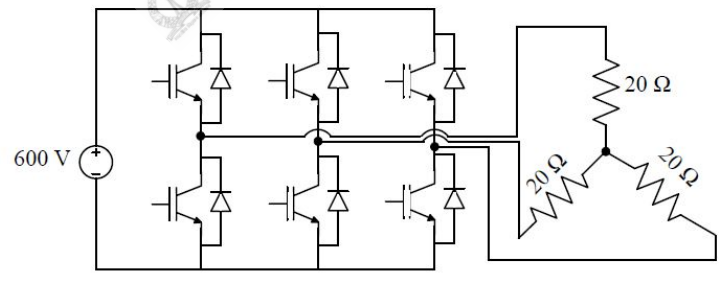
\includegraphics[width=0.5\textwidth]{figures/25.png}
\end{center}
\vspace{0.5cm}

\questionb{A function \( f(x) \) is defined as \( f(x) = \frac{\ln x + ax^2 + bx}{x - 1} \), where \( x \in \mathbb{R} \). Which one of the following statements is TRUE?}{26}
\begin{enumerate}
    \item[(A)] \( f(x) \) is NOT differentiable at \( x = 1 \) for any values of \( a \) and \( b \).  
    \item[(B)] \( f(x) \) is differentiable at \( x = 1 \) for the unique values of \( a \) and \( b \).  
    \item[(C)] \( f(x) \) is differentiable at \( x = 1 \) for all values of \( a \) and \( b \) such that \( a + b = e \).  
    \item[(D)] \( f(x) \) is differentiable at \( x = 1 \) for all values of \( a \) and \( b \).  
\end{enumerate}
\vspace{0.5cm}

\questionb{Consider the differential equation \( (t - 8)y'' + 5ty = \sin(t) \) with \( y(1) = 2 \). There exists a unique solution for this differential equation when \( t \) belongs to the interval}{27}
\begin{enumerate}
    \item[(A)] \( (-2, 2) \)  
    \item[(B)] \( (-10, 10) \)  
    \item[(C)] \( (-10, 2) \)  
    \item[(D)] \( (0, 10) \)  
\end{enumerate}
\vspace{0.5cm}

\questionb{Consider the line integral \( I = \int_C (x^2 + y^2) \, dz \), where \( z = x + iy \). The line \( C \) is shown in the figure below. The value of \( I \) is \_\_\_\_\_\_}{28}
\begin{center}
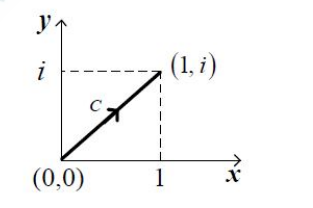
\includegraphics[width=0.5\textwidth]{figures/28.png}
\end{center}
\vspace{0.5cm}

\questionb{Two passive two-port networks are connected in cascade as shown in figure. A voltage source is connected at port 1. Given: \\
\( V_1 = A_1V_2 + B_1I_2 \), \( I_1 = C_1V_2 + D_1I_2 \) \\
\( V_2 = A_2V_3 + B_2I_3 \), \( I_2 = C_2V_3 + D_2I_3 \) \\
If the Thevenin equivalent circuit at port 3 consists of a voltage source \( V_T \) and an impedance \( Z_T \) connected in series, then}{29}
\begin{center}
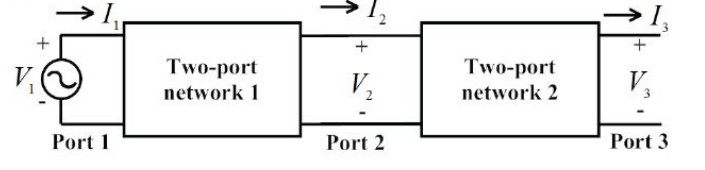
\includegraphics[width=0.5\textwidth]{figures/29.png}
\end{center}
\begin{enumerate}
    \item[(A)] \( V_T = \frac{V_1}{A_1B_2 + B_1D_2}, \quad Z_T = \frac{A_1A_2 + B_1C_2}{A_1B_2 + B_1D_2} \)  
    \item[(B)] \( V_T = \frac{V_1}{A_1B_2 + B_1D_2}, \quad Z_T = A_1 + A_2 \)  
    \item[(C)] \( V_T = \frac{V_1}{A_1A_2 + B_1C_2}, \quad Z_T = \frac{A_1A_2 + B_1C_2}{A_1B_2 + B_1D_2} \)  
    \item[(D)] \( V_T = \frac{V_1}{A_1A_2 + B_1C_2}, \quad Z_T = A_1 + A_2 \)  
\end{enumerate}
\vspace{0.5cm}

\questionb{Let a causal LTI system be characterized by the following differential equation with initial rest condition: \\
\[
\frac{d^2 y(t)}{dt^2} + 7 \frac{dy(t)}{dt} + 10 y(t) = 4x(t)
\] 
The impulse response of the system is (where \( u(t) \) is the unit step function)}{30}
\begin{enumerate}
    \item[(A)] \( 2e^{-2t}u(t) - 7e^{-5t}u(t) \)  
    \item[(B)] \( -2e^{-2t}u(t) + 7e^{-5t}u(t) \)  
    \item[(C)] \( 7e^{-2t}u(t) - 2e^{-5t}u(t) \)  
    \item[(D)] \( -7e^{-2t}u(t) + 2e^{-5t}u(t) \)  
\end{enumerate}
\vspace{0.5cm}

\questionb{Let the signal \( x(t) = \sum_{k=-\infty}^{\infty} (-1)^k \delta(t - 2kT) \) be passed through an LTI system with frequency response \( H(\omega) \), as given in the figure below. The Fourier series representation of the output is}{31}
\begin{center}
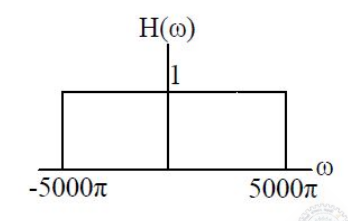
\includegraphics[width=0.5\textwidth]{figures/31.png}
\end{center}
\begin{enumerate}
    \item[(A)] \( 4000 + 4000\cos(2000\pi t) + 4000\cos(4000\pi t) \)  
    \item[(B)] \( 2000 + 2000\cos(2000\pi t) + 2000\cos(4000\pi t) \)  
    \item[(C)] \( 4000\cos(2000\pi t) \)  
    \item[(D)] \( 2000\cos(2000\pi t) \)  
\end{enumerate}
\vspace{0.5cm}

\questionb{In the system whose signal flow graph is shown in the figure, \( U_1(s) \) and \( U_2(s) \) are inputs. The transfer function is}{32}
\begin{center}
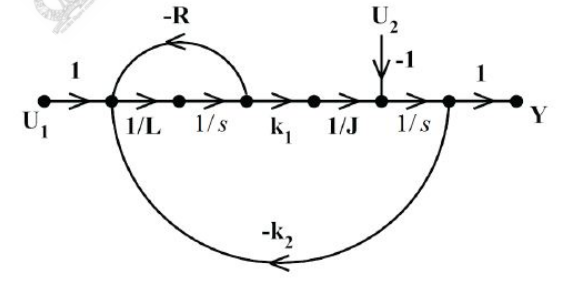
\includegraphics[width=0.5\textwidth]{figures/32.png}
\end{center}
\begin{enumerate}
    \item[(A)] \( \frac{k_y}{Js^2 + JR s + k_1k_2} \)  
    \item[(B)] \( \frac{k_y - U_1(R + sL)}{Js^2 + (JR - U_1L)s + k_1k_2 - U_1R} \)  
    \item[(C)] \( \frac{k_y - U_1(sL - R)}{Js^2 + (JR - U_1L)s + k_1k_2 - U_1R} \)  
    \item[(D)] \( \frac{JL^2 - (JR + U_1L)s - k_1k_2 + U_1R}{k_y} \)  
\end{enumerate}
\vspace{0.5cm}

\questionb{The transfer function of the system \( \frac{Y(s)}{U(s)} \) whose state-space equations are given below is: \\
\[
\begin{bmatrix}
\dot{x}_1(t) \\ \dot{x}_2(t)
\end{bmatrix}
=
\begin{bmatrix}
0 & 1 \\
-4 & -1
\end{bmatrix}
\begin{bmatrix}
x_1(t) \\ x_2(t)
\end{bmatrix}
+
\begin{bmatrix}
0 \\ 1
\end{bmatrix} u(t), \quad
y(t) = [1 \quad 0] \begin{bmatrix}
x_1(t) \\ x_2(t)
\end{bmatrix}
\]}{33}
\begin{enumerate}
    \item[(A)] \( \frac{1}{(s+2)(s-2)} \)  
    \item[(B)] \( \frac{1}{(s-4)(s+4)} \)  
    \item[(C)] \( \frac{1}{s^2 + s - 4} \)  
    \item[(D)] \( \frac{1}{s^2 - s - 4} \)  
\end{enumerate}
\vspace{0.5cm}

\questionb{The load shown in the figure is supplied by a 400 V (line-to-line), 3-phase source (RYB sequence). The load is balanced and inductive, drawing 3464 VA. When the switch \( S \) is in position \( N \), the three watt-meters \( W_1, W_2 \) and \( W_3 \) read 577.35 W each. If the switch is moved to position \( Y \), the readings of the watt-meters in watts will be:}{34}
\begin{center}
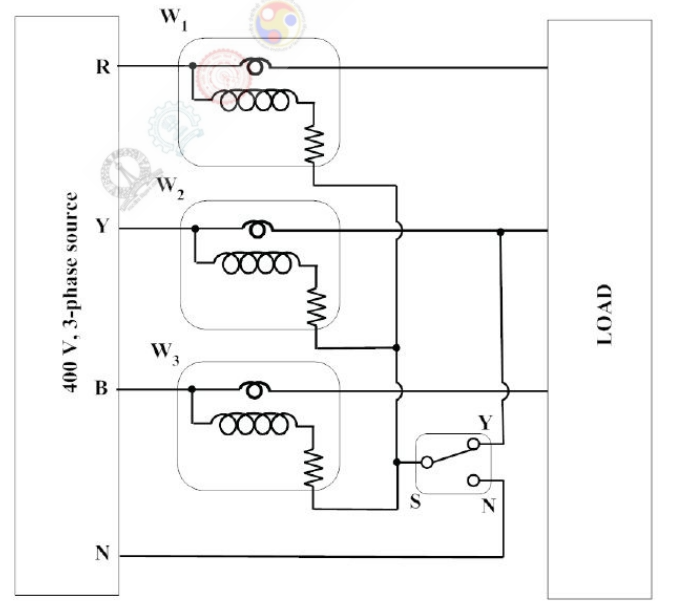
\includegraphics[width=0.5\textwidth]{figures/34.png}
\end{center}
\begin{enumerate}
    \item[(A)] \( W_1 = 1732 \) and \( W_2 = W_3 = 0 \)  
    \item[(B)] \( W_1 = 0, W_2 = 1732 \) and \( W_3 = 0 \)  
    \item[(C)] \( W_1 = 0, W_2 = 0 \) and \( W_3 = 1732 \)  
    \item[(D)] \( W_1 = W_2 = W_3 = 577.35 \)  
\end{enumerate}
\vspace{0.5cm}

\questionb{The approximate transfer characteristic for the circuit shown below with an ideal operational amplifier and diode will be}{35}
\begin{center}
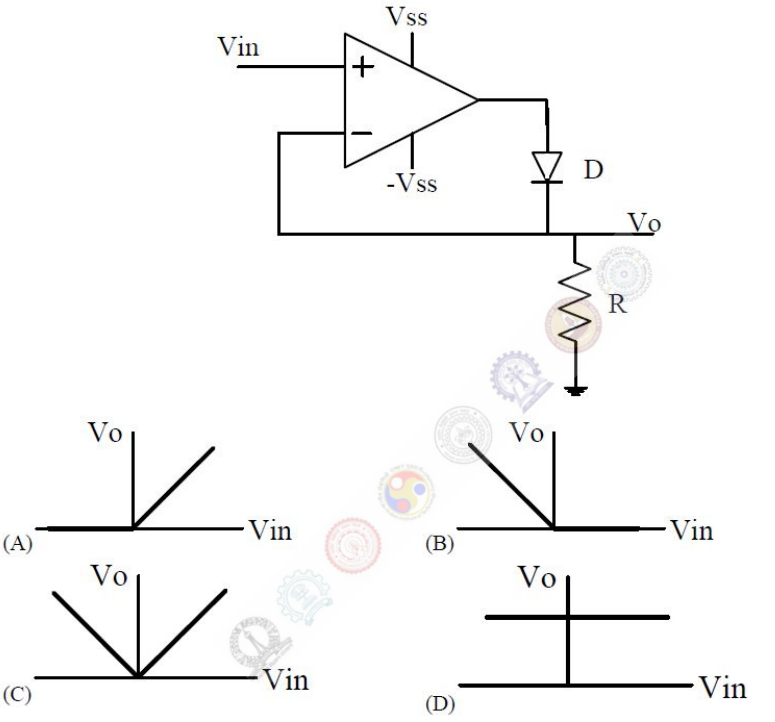
\includegraphics[width=0.9\textwidth]{figures/35.png}
\end{center}
\vspace{0.5cm}

\questionb{The output expression for the Karnaugh map shown below is}{36}
\begin{center}
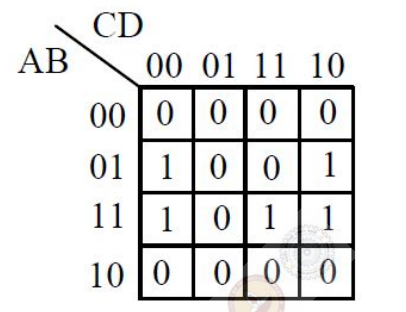
\includegraphics[width=0.5\textwidth]{figures/36.png}
\end{center}
\begin{enumerate}
    \item[(A)] \( BD + BCD \)  
    \item[(B)] \( BD + AB \)  
    \item[(C)] \( BD + ABC \)  
    \item[(D)] \( BD + ABC \)  
\end{enumerate}
\vspace{0.5cm}

\questionb{The logical gate implemented using the circuit shown below where, \( V_1 \) and \( V_2 \) are inputs (with 0 V as digital 0 and 5 V as digital 1) and \( V_{OUT} \) is the output, is}{37}
\begin{center}
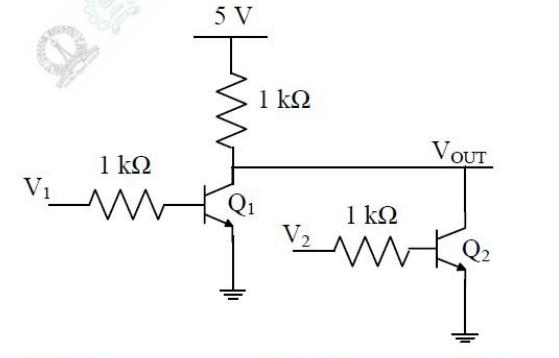
\includegraphics[width=0.5\textwidth]{figures/37.png}
\end{center}
\begin{enumerate}
    \item[(A)] NOT  
    \item[(B)] NOR  
    \item[(C)] NAND  
    \item[(D)] XOR  
\end{enumerate}
\vspace{0.5cm}

\questionb{The input voltage \( V_{in} \) of the buck-boost converter shown below varies from 32 V to 72 V. Assume that all components are ideal, inductor current is continuous, and output voltage is ripple free. The range of duty ratio \( D \) of the converter for which the magnitude of the steady-state output voltage remains constant at 48 V is}{38}
\begin{center}
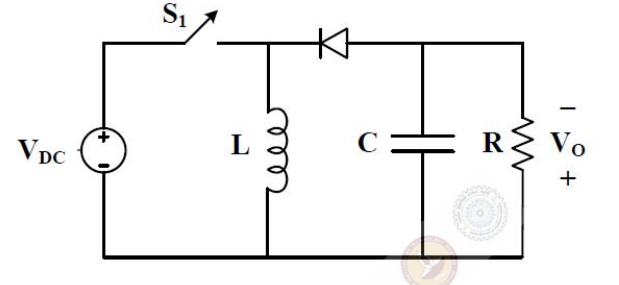
\includegraphics[width=0.5\textwidth]{figures/38.png}
\end{center}
\begin{enumerate}
    \item[(A)] \( \frac{2}{5} \leq D \leq \frac{3}{5} \)  
    \item[(B)] \( \frac{2}{3} \leq D \leq 1 \)  
    \item[(C)] \( \frac{1}{2} \leq D \leq \frac{3}{4} \)  
    \item[(D)] \( \frac{1}{3} \leq D \leq \frac{2}{3} \)  
\end{enumerate}
\vspace{0.5cm}

\questionb{A load is supplied by a 230 V, 50 Hz source. The active power \( P \) and the reactive power \( Q \) consumed by the load are such that \( 1 \text{ kW} < P < 2 \text{ kW} \) and \( 1 \text{ kVAR} \leq Q < 2 \text{ kVAR} \). A capacitor connected across the load for power factor correction generates 1 kVAR reactive power. The worst case power factor after power factor correction is}{39}
\begin{enumerate}
    \item[(A)] 0.447 lag  
    \item[(B)] 0.707 lag  
    \item[(C)] 0.894 lag  
    \item[(D)] 1  
\end{enumerate}
\vspace{0.5cm}

\questionb{The bus admittance matrix for a power system network is \\
\[
\begin{bmatrix}
-j39.9 & j20 & j20 \\
j20 & -j39.9 & j20 \\
j20 & j20 & -j39.9
\end{bmatrix} \, \text{pu}
\] 
There is a transmission line, connected between buses 1 and 3, which is represented by the circuit shown in figure. Reactance is 0.05 pu. Susceptance is 0.05 pu. If this transmission line is removed from service, what is the modified bus admittance matrix?}{40}
\begin{center}
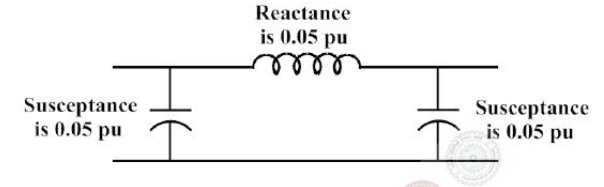
\includegraphics[width=0.5\textwidth]{figures/40.png}
\end{center}
\begin{enumerate}
    \item[(A)] 
    \(
    \begin{bmatrix}
    -j19.9 & j20 & 0 \\
    j20 & -j39.9 & j20 \\
    0 & j20 & -j19.9
    \end{bmatrix}
    \) pu  
    \item[(B)] 
    \(
    \begin{bmatrix}
    -j39.9 & j20 & 0 \\
    j20 & -j39.9 & j20 \\
    0 & j20 & -j39.9
    \end{bmatrix}
    \) pu  
    \item[(C)] 
    \(
    \begin{bmatrix}
    -j19.95 & j20 & 0 \\
    j20 & -j39.9 & j20 \\
    0 & j20 & -j19.95
    \end{bmatrix}
    \) pu  
    \item[(D)] 
    \(
    \begin{bmatrix}
    -j39.9 & j20 & j20 \\
    j20 & -j39.9 & j20 \\
    j20 & j20 & -j39.9
    \end{bmatrix}
    \) pu  
\end{enumerate}
\vspace{0.5cm}

\questionb{The switch in the figure below was closed for a long time. It is opened at \( t = 0 \). The current in the inductor of 2 H for \( t = 0^+ \) is}{41}
\begin{center}
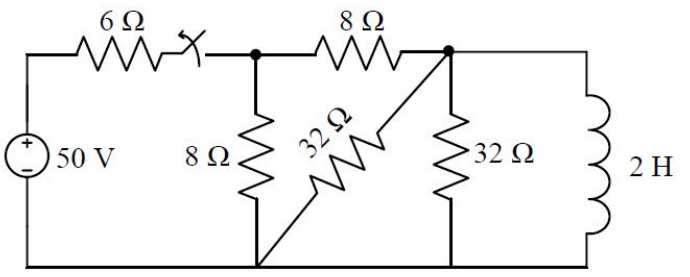
\includegraphics[width=0.5\textwidth]{figures/41.png}
\end{center}
\begin{enumerate}
    \item[(A)] \( 2.5e^{-4t} \)  
    \item[(B)] \( 5e^{-4t} \)  
    \item[(C)] \( 2.5e^{-0.25t} \)  
    \item[(D)] \( 5e^{-1.25t} \)  
\end{enumerate}
\vspace{0.5cm}

\questionb{Only one of the real roots of \( f(x) = x^3 - x - 1 \) lies in the interval \( 1 \leq x \leq 2 \) and bisection method is used to find its value. For achieving an accuracy of 0.001, the required minimum number of iterations is \_\_\_\_\_\_}{42}
\vspace{0.5cm}

\questionb{In the circuit shown below, the maximum power transferred to the resistor \( R \) is \_\_\_\_\_\_ W.}{43}
\begin{center}
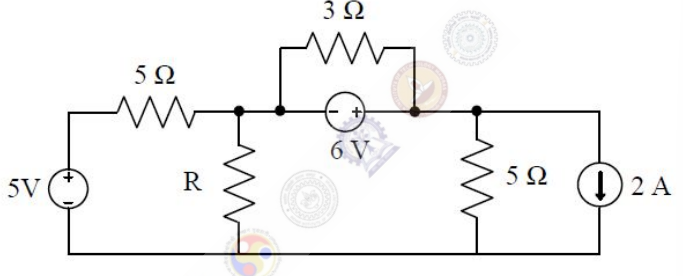
\includegraphics[width=0.5\textwidth]{figures/43.png}
\end{center}
\vspace{0.5cm}

\questionb{The magnitude of magnetic flux density \( B \) in micro Teslas (\( \mu T \)) at the center of a loop of wire wound as a regular hexagon of side length 1 m carrying a current \( I = 1 \) A and placed in vacuum as shown in the figure is \_\_\_\_\_\_ (Give the answer up to two decimal places.)}{44}
\begin{center}
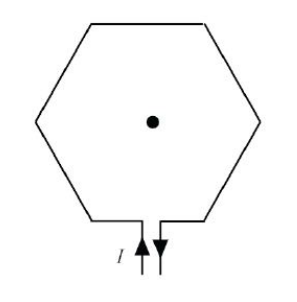
\includegraphics[width=0.5\textwidth]{figures/44.png}
\end{center}
\vspace{0.5cm}

\questionb{A 375 W, 230 V, 50 Hz capacitor start single-phase induction motor has the following constants for the main and auxiliary windings (at starting): \( Z_m = (12.50 + j15.75)\,\Omega \) (main winding), \( Z_a = (24.50 + j12.75)\,\Omega \) (auxiliary winding). Neglecting the magnetizing branch, the value of the capacitance (in \( \mu F \)) to be added in series with the auxiliary winding to obtain maximum torque at starting is \_\_\_\_\_\_}{45}
\vspace{0.5cm}

\questionb{Two parallel connected, three-phase, 50 Hz, 11 kV, star-connected synchronous machines A and B are operating as synchronous condensers. They together supply 50 MVAR to a 11 kV grid. Currents supplied by both the machines are equal. Synchronous reactances of machine A and machine B are 1 \( \Omega \) and 3 \( \Omega \), respectively. Assuming the magnetic circuit to be linear, the ratio of excitation current of machine A to that of machine B is \_\_\_\_\_\_ (Give the answer up to two decimal places.)}{46}
\vspace{0.5cm}

\questionb{A 220 V DC series motor runs drawing a current of 30 A from the supply. Armature and field circuit resistances are 0.4 \( \Omega \) and 0.1 \( \Omega \), respectively. The load torque varies as the square of the speed. The flux in the motor may be taken as being proportional to the armature current. To reduce the speed of the motor by 50\%, the resistance in ohms that should be added in series with the armature is \_\_\_\_\_\_ (Give the answer up to two decimal places.)}{47}
\vspace{0.5cm}

\questionb{A three-phase, three winding \( \Delta/\Delta/Y \) (1.1 kV / 6.6 kV / 400 V) transformer is energized from AC mains at the 1.1 kV side. It supplies 900 kVA load at 0.8 power factor lag from the 6.6 kV winding and 300 kVA load at 0.6 power factor lag from the 400 V winding. The RMS line current in ampere drawn by the 1.1 kV winding from the mains is \_\_\_\_\_\_ (Give the answer up to one decimal place.)}{48}
\vspace{0.5cm}

\questionb{A separately excited DC generator supplies 150 A to a 145 V DC grid. The generator is running at 800 RPM. The armature resistance of the generator is 0.1 \( \Omega \). If the speed of the generator is increased to 1000 RPM, the current in amperes supplied by the generator to the DC grid is \_\_\_\_\_\_ (Give the answer up to one decimal place.)}{49}
\vspace{0.5cm}

\questionb{For a system having transfer function \( G(s) = \frac{s+1}{s+2} \), a unit step input is applied at time \( t = 0 \). The value of the response of the system at \( t = 1.5 \) sec (rounded off to three decimal places) is \_\_\_\_\_\_}{50}
\vspace{0.5cm}

\questionb{Consider a causal and stable LTI system with rational transfer function \( H(z) \), whose corresponding impulse response begins at \( n = 0 \). Furthermore, \( H(1) = \frac{1}{\sqrt{2}} \). The poles of \( H(z) \) are \( z_k = \exp\left(j(2k + 1)\frac{\pi}{4}\right) \) for \( k = 1, 2, 3, 4 \). The zeros of \( H(z) \) are all at \( z = 0 \). Let \( g[n] = h[n] * h[n] \). The value of \( g[8] \) equals \_\_\_\_\_\_ (Give the answer up to three decimal places.)}{51}
\vspace{0.5cm}

\questionb{The circuit shown in the figure uses matched transistors with a thermal voltage \( V_T = 25 \) mV. The base currents of the transistors are negligible. The value of the resistance \( R \) in \( \text{k}\Omega \) that is required to provide 1 \( \mu \)A bias current for the differential amplifier block shown is \_\_\_\_\_\_ (Give the answer up to one decimal place.)}{52}
\begin{center}
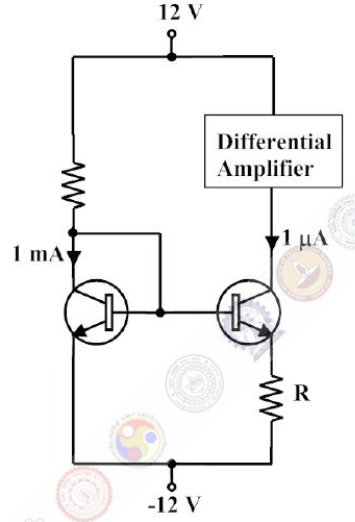
\includegraphics[width=0.5\textwidth]{figures/52.png}
\end{center}
\vspace{0.5cm}

\questionb{The figure below shows an uncontrolled diode bridge rectifier supplied from a 220 V, 50 Hz, 1-phase AC source. The load draws a constant current \( I_0 = 14 \) A. The conduction angle of the diode \( D_1 \) in degrees (rounded off to two decimal places) is \_\_\_\_\_\_}{53}
\begin{center}
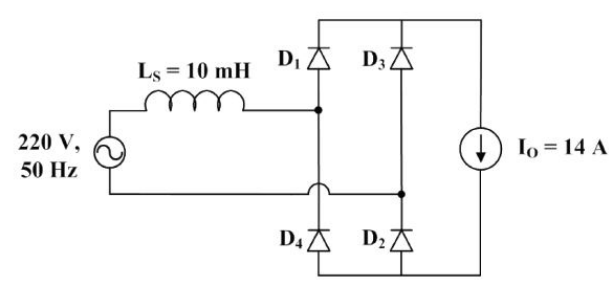
\includegraphics[width=0.5\textwidth]{figures/53.png}
\end{center}
\vspace{0.5cm}

\questionb{The positive, negative, and zero sequence reactances of a wye-connected synchronous generator are 0.2 pu, 0.2 pu, and 0.1 pu, respectively. The generator is on open circuit with a terminal voltage of 1 pu. The minimum value of the inductive reactance, in pu, required to be connected between neutral and ground so that the fault current does not exceed 3.75 pu if a single line to ground fault occurs at the terminals is \_\_\_\_\_\_ (assume fault impedance to be zero) (Give the answer up to one decimal place.)}{54}
\vspace{0.5cm}

\questionb{The figure shows the single line diagram of a power system with a double circuit transmission line. The expression for electrical power is \( 1.5\sin\delta \), where \( \delta \) is the rotor angle. The system is operating at the stable equilibrium point with mechanical power equal to 1 pu. If one of the transmission line circuits is removed, the maximum value of \( \delta \), as the rotor swings, is 1.221 radians. If the expression for electrical power with one transmission line circuit removed is \( B_1 \sin\delta \), the value of \( B_1 \), in pu, is \_\_\_\_\_\_ (Give the answer up to three decimal places.)}{55}
\begin{center}
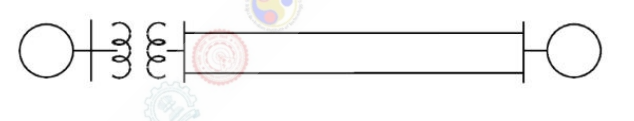
\includegraphics[width=0.5\textwidth]{figures/55.png}
\end{center}
\vspace{0.5cm}


\vspace{5cm}
\begin{center}
\textbf{END OF THE QUESTION PAPER} \\
\rule{\textwidth}{0.5pt}
\end{center}

\end{document}
